\documentclass[12pt]{scrartcl}

\usepackage[utf8]{inputenc}
\usepackage[IL2]{fontenc}
\usepackage[czech]{babel}
\usepackage{graphicx}
\usepackage{hyperref}
\usepackage{amsmath}
\usepackage[]{algorithm2e}
\usepackage{enumitem}

\subject{Západočeská univerzita v\nobreakspace Plzni\\Fakulta aplikovaných věd\\KIV/KPG}
\author{Pavel Zelenka\\A16B0176P\\zelenkap@students.zcu.cz}
\date{\today}
\title{Bludiště}

\begin{document}
\maketitle
\pagenumbering{gobble}
\newpage
\pagenumbering{arabic}
\newpage
\section{Zadání}
	
\paragraph{}
Zadáním úkolu je vytvoření programu generujícího a\nobreakspace vykreslujícího bludiště. 

\section{Analýza problému}

\paragraph{}
\textbf{Bludiště} je hlavolam, ve\nobreakspace kterém existuje alespoň jedna cesta od\nobreakspace startu k\nobreakspace cíly. Úkolem řešitele je\nobreakspace tuto cestu najít. Cesty v\nobreakspace bludišti od\nobreakspace sebe oddělují zdi, skrze které nelze procházet. 
\paragraph{}
Bludiště lze rozdělit na\nobreakspace políčka, které budou reprezentovat část bludiště a\nobreakspace budou uchovávat informace o\nobreakspace průchodech. Tento způsob lze implementovat číselnou maticí, která bude mít vyhrazenu jednu číslici pro zeď (např.\nobreakspace 0) a\nobreakspace druhou pro cestu (např.\nobreakspace 1). V\nobreakspace případě, že bude potřebné uchovávat i\nobreakspace další informace, lze políčka bludiště implementovat založením nové třídy a\nobreakspace matice bludiště bude místo čísel obsahovat instance této třídy. 
\paragraph{}
Při generování bludiště bude nutné rozpoznat políčka, které již jsou připojeny do\nobreakspace cesty a\nobreakspace políčka, které zatím na\nobreakspace připojení čekají. Při implementaci číselnou maticí lze zavést třetí číslici označující zatím neprocházené políčko (např.\nobreakspace -1). V\nobreakspace případě implementace třídou reprezentující políčko se nabízí několik způsovů, například uchováváním vzdálenosti od\nobreakspace startu, referencemi na sousední políčka či\nobreakspace Booleovou proměnnou.
\paragraph{}
Vytváření cest lze naprogramovat skrze rekurzivní metodu, které se\nobreakspace zadá jen počáteční políčko bludiště. Procházené políčko bude muset znát sousední políčka, když bude existovat sousední políčko, které zatím není napojeno do\nobreakspace žádné cesty, lze jej napojit.
\paragraph{}
Cíl bludiště by\nobreakspace nebylo vhodné umístit blízko startu, proto bude dobré\nobreakspace si uchovávat vzdálenost od\nobreakspace startu pro každé políčko a\nobreakspace zvolit jako cílové políčko s\nobreakspace největší možnou vzdáleností.

\newpage
\section{Popis řešení}

\paragraph{}
Aplikace se skládá z celkem 7 tříd.
\begin{itemize}[noitemsep] 
\item Třída \emph{MainMaze} je hlavní třídou aplikace.
\item Třída \emph{Drawing} se stará o vykreslování bludiště.
\item Třída \emph{Maze} generuje a uchovává matici bludiště.
\item Třída \emph{Cell} uchovává podrobnosti políčka bludiště.
\item Třída \emph{Player} uchovává pozici hráče.
\item Třída \emph{PlayerController} zpracovává události z klávesnice.
\item Třída \emph{WindowLayout} popisuje grafické uživatelské rozhraní aplikace.
\end{itemize}

\paragraph{}
Po spuštění aplikace se zavolá konstruktor třídy \emph{Drawing}, který vytvoří novou instanci třídy \emph{Maze}. Při vytváření instance třídy \emph{Maze} zavolá metoda \emph{generateSurface}, která vytvoří matici políček třídy \emph{Cell} reprezentující plochu bludiště. Skrze rekurzivně fungující metodu \emph{createPaths} se vytvoří cesta v bludišti. 

\paragraph{}
\begin{algorithm}[H]
	\BlankLine
	označ procházené políčko jako připojené do cesty
	\BlankLine
	\While{existuje nepřipojené sousední políčko}{
		\BlankLine
		připoj procházené políčko s nepřipojeným sousedním políčkem
		\BlankLine
		nastav vzdálenost sousedního políčka od startu o 1 vyšší než má současné políčko
		\BlankLine
		spusť tento algoritmus na sousedním políčku
		\BlankLine
	}
 \caption{Rekurzivní vytváření cesty v bludišti}
\end{algorithm}

\paragraph{}
Po vytvoření bludiště následuje vytvoření hráče, který je umístěn na startovní políčko. Ovládání obsluhuje třída \emph{PlayerController}, která se aktivuje zavoláním metody \emph{activation} po nastavení hráče, scény a kresby. Po aktivaci třída zpracovává vstupy z klávesnice. V případě, že v době stisku klávesy běží animace, tak se událost uloží do fronty a zpracuje se skončení animace. 

\paragraph{}
\begin{algorithm}[H]
	\eIf{animace běží}
		{přidej událost stisku klávesy do fronty}
		{
			zjisti možné pohyby hráče
			\BlankLine
			\If{je požadován možný pohyb} {
				změň pozici hráče
			}
		}
 \caption{Zpracování vstupu z klávesnice}
\end{algorithm}

\section{Uživatelská dokumentace}
\paragraph{}
Aplikace byla testována na operačním systému \textbf{GNU/Linux} s nainstalovaným \textbf{Java Development Kit} ve\nobreakspace verzi\nobreakspace 1.8.0\_162.
Spuštění aplikace se\nobreakspace provede souborem \texttt{Maze.jar}, který se nachází ve složce \emph{App}.

\paragraph{}
Po\nobreakspace spuštění aplikace se\nobreakspace zobrazí okno ve\nobreakspace kterém bude vygenerované bludiště. Startovací pozice je\nobreakspace vyobrazena oranžovou barvou, cílová pozice je vyobrazena zeleně. Pozici hráče reprezentuje červené kolečko. Aplikace se ovládá šipkami na\nobreakspace klávesnici. V\nobreakspace případě dosažení cíle se\nobreakspace vygeneruje nová mapa, která bude o\nobreakspace jeden sloupec a\nobreakspace jeden řádek větší.

\begin{figure}[!ht]
	\centering
	\label{obr:polekolizi}
	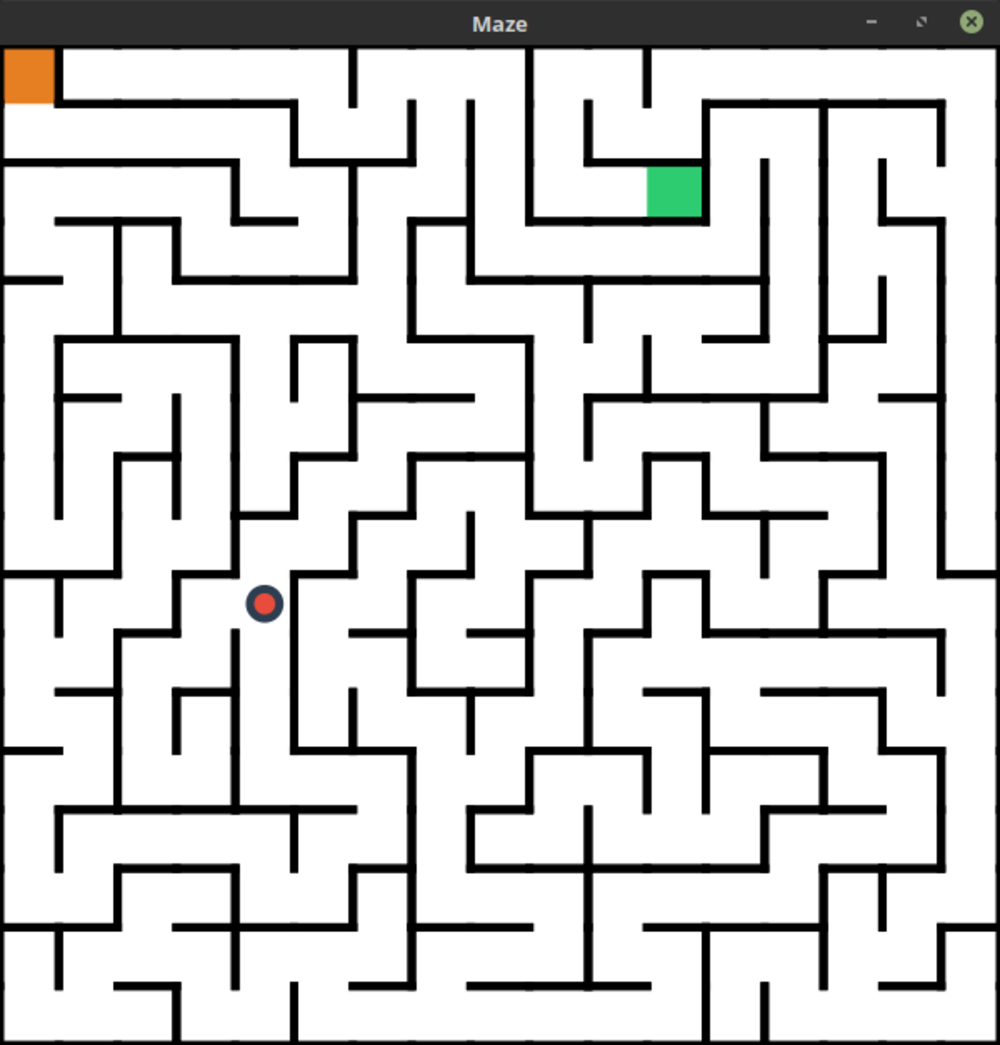
\includegraphics[width=0.9\textwidth,natwidth=1,natheight=1]{app_gui.pdf}
	\caption{Okno aplikace}
\end{figure}	

\newpage
\section{Závěr}
\paragraph{}
Úkol jsem řešil v\nobreakspace jazyce \texttt{Java} s použitím grafických knihoven \texttt{JavaFX}.
Aplikace v\nobreakspace odevzdávané podobě uživateli nijak neumožňuje provést změnu parametrů bludiště. Přidání možnosti nastavení parametrů by neměl být problém, protože aplikace je psaná z\nobreakspace ohledem na snadné změny klíčových parametrů. Plátno je umístěné ve\nobreakspace střední pozici v\nobreakspace \texttt{BorderPane}, který umožňuje přidání dalších panelů kolem bludiště.

\section{Reference}

Bludiště – Wikipedie. [online]. Dostupné z: \href{https://cs.wikipedia.org/wiki/Bludiště}{cs.wikipedia.org/wiki/Bludiště}

\end{document}
